%%%%%%%%%%%%%%%%%%%%%%%%%%%%%%%%%%%%%%%%%
% Programming/Coding Assignment
% LaTeX Template
%
% This template has been downloaded from:
% http://www.latextemplates.com
%
% Original author:
% Ted Pavlic (http://www.tedpavlic.com)
%
% Note:
% The \lipsum[#] commands throughout this template generate dummy text
% to fill the template out. These commands should all be removed when 
% writing assignment content.
%
% This template uses a Perl script as an example snippet of code, most other
% languages are also usable. Configure them in the "CODE INCLUSION 
% CONFIGURATION" section.
%
%%%%%%%%%%%%%%%%%%%%%%%%%%%%%%%%%%%%%%%%%

%----------------------------------------------------------------------------------------
%	PACKAGES AND OTHER DOCUMENT CONFIGURATIONS
%----------------------------------------------------------------------------------------

\documentclass{article} 

\usepackage{fancyhdr} % Required for custom headers
\usepackage{lastpage} % Required to determine the last page for the footer
\usepackage{extramarks} % Required for headers and footers
\usepackage[usenames,dvipsnames]{color} % Required for custom colors
\usepackage{graphicx} % Required to insert images
\usepackage{listings} % Required for insertion of code
\usepackage{courier} % Required for the courier font
\usepackage{multirow}
\usepackage{hyperref}
\usepackage{amsmath}
\usepackage{amssymb}


% Margins
\topmargin=-0.45in
\evensidemargin=0in
\oddsidemargin=0in
\textwidth=6.5in
\textheight=9.0in
\headsep=0.25in

\linespread{1.1} % Line spacing

%----------------------------------------------------------------------------------------
%	CODE INCLUSION CONFIGURATION
%----------------------------------------------------------------------------------------

\definecolor{MyDarkGreen}{rgb}{0.0,0.4,0.0} % This is the color used for comments
\lstloadlanguages{c} % Load Perl syntax for listings, for a list of other languages supported see: ftp://ftp.tex.ac.uk/tex-archive/macros/latex/contrib/listings/listings.pdf
\lstset{language=[sharp]c, % Use Perl in this example
        frame=single, % Single frame around code
        basicstyle=\small\ttfamily, % Use small true type font
        keywordstyle=[1]\color{Blue}\bf, % Perl functions bold and blue
        keywordstyle=[2]\color{Purple}, % Perl function arguments purple
        keywordstyle=[3]\color{Blue}\underbar, % Custom functions underlined and blue
        identifierstyle=, % Nothing special about identifiers                                         
        commentstyle=\usefont{T1}{pcr}{m}{sl}\color{MyDarkGreen}\small, % Comments small dark green courier font
        stringstyle=\color{Purple}, % Strings are purple
        showstringspaces=false, % Don't put marks in string spaces
        tabsize=5, % 5 spaces per tab
        %
        % Put standard Perl functions not included in the default language here
        morekeywords={rand},
        %
        % Put Perl function parameters here
        morekeywords=[2]{on, off, interp},
        %
        % Put user defined functions here
        morekeywords=[3]{test},
       	%
        morecomment=[l][\color{Blue}]{...}, % Line continuation (...) like blue comment
        numbers=left, % Line numbers on left
        firstnumber=1, % Line numbers start with line 1
        numberstyle=\tiny\color{Blue}, % Line numbers are blue and small
        stepnumber=5 % Line numbers go in steps of 5
}

\newcommand{\horrule}[1]{\rule{\linewidth}{#1}}

% Creates a new command to include a perl script, the first parameter is the filename of the script (without .pl), the second parameter is the caption
\newcommand{\perlscript}[2]{
\begin{itemize}
\item[]\lstinputlisting[caption=#2,label=#1]{#1.cs}
\end{itemize}
}

\begin{document}

\begin{tabular}{l l}
\multirow{5}{*}{
\includegraphics[width=2cm]{../recursos/logo.png}} & Universidad del Istmo de Guatemala \\
 & Facultad de Ingenieria \\
 & Ing. en Sistemas \\
 & Informatica 1 \\
 & Prof. Ernesto Rodriguez - \href{mailto:erodriguez@unis.edu.gt}{erodriguez@unis.edu.gt} \\
\end{tabular}
\\\\\\

\begin{center}
        \horrule{0.5pt}
        \huge{Proyecto Final: Fractales} \\
        \large{Fecha de entrega: 28 de Octubre, 2019 - 11:59pm} \\
        \horrule{1pt}
\end{center}

\emph{Instrucciones: Resolver cada uno de los ejercicios siguiendo sus respectivas
instrucciones. El trabajo debe ser entregado a traves de Github, en su repositorio del curso, colocado en una carpeta llamada "Proyecto Final".
Al menos que la pregunta indique diferente, todas las respuestas a preguntas escritas deben presentarse en
un documento formato pdf, el cual haya sido generado mediante Latex. }
\\\\
A continuaci\'on se presenta el proyecto final. El objetivo de este proyecto es familiarizar al
estudiante con la utilizaci\'on de la programaci\'on funcional para crear programas interactivos.
El objetivo es que el estudiante construya un programa que dibuje fractales.
\\\\
El proyecto se puede llevar a en grupos de un maximo de 3 integrantes. Este proyecto tiene como valor 15 puntos
de los 40 que conforman el examen final. Adicionalmente, existe la oportunidad de 15 puntos extra de los cuales 5
seran para el examen final y 10 para recuperar nota en los parciales anteriores.
\\\\
Aparte de la entrega final, el dia 29 de Octubre, tendra que presentarle el codigo
al profesor durante la clase. El profesor tiene derecho de hacerle preguntas sobre
cualquier parte del codigo a cualquiera de los integrantes del grupo. La nota final
del proyecto es individual (no grupal) y dependera de la habilidad de cada integrante
en responder las preguntas que el profesor le haga sobre el codigo.

\section*{Copo de Nieve de Koch (5pts)}
\begin{center}
    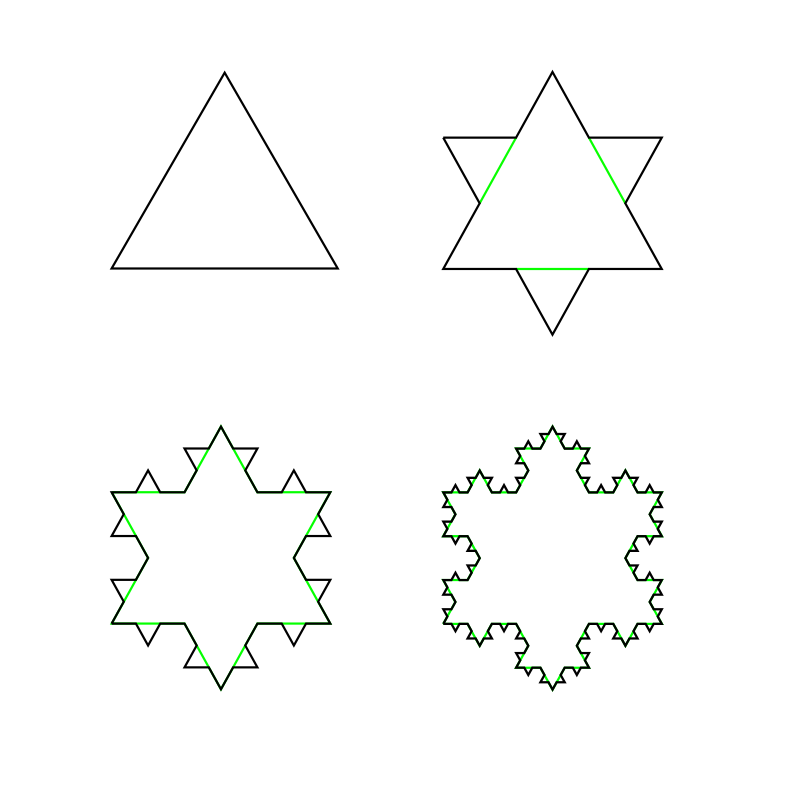
\includegraphics[width=5cm]{include/koch.png}
\end{center}
El copo de nieve de Koch (\url{https://en.m.wikipedia.org/wiki/Koch_snowflake}) es un poligono definido recursivamente.
Dado un poligono (un triangulo por ejemplo), se puede generar el
siguiente poligono asi:
\begin{enumerate}
        \item{Dividir cada linea del poligono en 3 partes exactas.}
        \item{Crear un triangulo nuevo en el espacio abarcado por la linea del medio
        \begin{itemize}
                \item{La longitud de cada linea del triangulo nuevo es la misma que la
                linea del medio.}
        \end{itemize}
        }
\end{enumerate}
Su tarea consiste en definir una funci\'on llamada $\mathtt{snowflake}\ :\ \mathbb{N}\rightarrow
\mathtt{List}\ (\mathbb{R},\mathbb{R})$. Esta funci\'on debe aceptar un numero natural indicando
la cantidad de veces que se repetira la recursion. El valor 0 representa el copo m\'as simple
de Koch (un tirangulo) y numeros mayores a 0 representan la cantidad de repetici\'ones que se
llevaran a cabo en la producci\'on del copo de nieve. El resultado de esta funci\'on es una
lista de parejas de numeros reales ($\mathbf{Float}$) que representan los vertices del copo
de nieve en un plano cartesiano de coordenadas.

\section*{Triangulo de Sierpinski (5pts)}
%%\begin{center}
%%        \includegraphics[width=5cm]{include/sierpinski.jpg}
%%\end{center}
El triangulo de Sierpinski (\url{https://en.wikipedia.org/wiki/Sierpinski_triangle}) es otro fractal generado recursivamente.
El caso base consiste en un triangulo regular. Luego, cada paso recursivo divide cada uno de los triangulos que
conforman el triangulo mediante otro triangulo que cada lado del triangulo esta ubicado en
la mitad de cada una de las lineas del triangulo anterior.
\\\\
Su tarea consiste en definir la funci\'on $\mathtt{sierpinski}\ :\ \mathbb{N}\rightarrow \mathtt{List}\ 
(\mathtt{List}\ (\mathbb{R}, \mathbb{R}))$ la cual debe aceptar un numero natural como parametro y generar
una lista de listas de parejas de numeros reales. La interpretaci\'on de este resultado es que cada
lista de numeros corresponde a uno de los muchos triangulos que conforman el triangulo de Sierpinsky. 

\section*{Visualizaci\'on (5pts)}

Utilizar el modulo Html y Canvas de Elm para crear una interfaz grafica que permita visualizar el
triangulo de Sierpinski y el copo de Koch. Esta interfaz debe tener lo siguiente:
\begin{itemize}
    \item{Un campo para seleccionar el fractal que se desea dibujar}
    \item{Un campo para seleccionar el numero de repeticiones que se utilizar
    para crear el fractal.}
    \item{Un area donde el poligono seleccionado es dibujado}
\end{itemize}

Esta interfaz debe ser interactiva, lo que significa que se pueden modificar
los valores y area de visualizaci\'on dibuja el factal con los parametros
actualizados.

\section*{Extras (15pts)}
Se otorgaran hasta 15 puntos extras por articulos adicionales en la entrega que esten relacionados
al trabajo. Algunos ejemplos podrian ser:
\begin{itemize}
        \item{Utilizar css para mejorar la apariencia visual del programa}
        \item{Inclusion de otros fractales}
        \item{Fractales de 3 o m\'as dimensiones}
        \item{Utilizar color diferente para cada recursion dibujada para mejor
        visualizacion del fractal.}
        \item{Opcion de dibujar el fractal de forma probabilistica. Ie. a los
        puntos que conforman las esquians del fractal se les modifica la posici\'on
        ligeramente mediante numeros aleatoreos.}
        \item{Interactividad con el mouse}
        \item{Cualquier cosa extra que usted se imagine, discutir con migo
        si desea saber exactametne el puntaje que se dara por su extra.}
\end{itemize}

\section*{Proyectos Alternativos}

Se aceptan propuestas para proyectos alternativos. Se requiere que los proyectos
involucren los temas aprendidos en clase, por lo cual se debe utilizar un
\emph{lenguaje puramente funcional} como Elm, Haskell, OCaml, SML, Prolog o Agda.

Es possible negociar aun m\'as puntos extras (adicionales al 15\% extra) si su proyecto
tiene como resultado un aporte a la comunidad de software libre (open-source). Si
lo desea, puede buscar en Google Summer of Code \url{summerofcode.withgoogle.com}
ideas de proyectos.

\end{document}